% Preamble templated from Mihir-Divyansh/Course-Setup
%iffalse
\let\negmedspace\undefined
\let\negthickspace\undefined
\documentclass[journal,12pt,onecolumn]{IEEEtran}
\usepackage{cite}
\usepackage{amsmath,amssymb,amsfonts,amsthm}
\usepackage{algorithmic}
\usepackage{graphicx}
\usepackage{textcomp}
\usepackage{xcolor}
\usepackage{txfonts}
\usepackage{listings}
\usepackage{enumitem}
\usepackage{mathtools}
\usepackage{gensymb}
\usepackage{comment}
\usepackage[breaklinks=true]{hyperref}
\usepackage{tkz-euclide}
\usepackage{listings}
\usepackage{gvv}
%\def\inputGnumericTable{}
\usepackage[latin1]{inputenc}
\usepackage{color}
\usepackage{array}
\usepackage{longtable}
\usepackage{calc}
\usepackage{multirow}
\usepackage{hhline}
\usepackage{ifthen}
\usepackage{lscape}
\usepackage{tabularx}
\usepackage{array}
\usepackage{float}
\usepackage{caption}
\usepackage{multicol}

\newtheorem{theorem}{Theorem}[section]
\newtheorem{problem}{Problem}
\newtheorem{proposition}{Proposition}[section]
\newtheorem{lemma}{Lemma}[section]
\newtheorem{corollary}[theorem]{Corollary}
\newtheorem{example}{Example}[section]
\newtheorem{definition}[problem]{Definition}
\newcommand{\BEQA}{\begin{eqnarray}}
\newcommand{\EEQA}{\end{eqnarray}}
%\newcommand{\define}{\stackrel{\triangle}{=}}
\theoremstyle{remark}
%\newtheorem{rem}{Remark}

% Marks the beginning of the document
\begin{document}
\bibliographystyle{IEEEtran}
\vspace{3cm}

\title{Assignment 11: 5.5.7}
\author{EE25BTECH11055 - Subhodeep Chakraborty}
\maketitle
\hrulefill
\bigskip

\renewcommand{\thefigure}{\theenumi}
\renewcommand{\thetable}{\theenumi}

\textbf{Question:}\par
Find the inverse of the following matrix, using elementary transformations\hfill\brak{12, 2019}
$$\myvec{2&3&1\\2&4&1\\3&7&2}$$
\par
\textbf{Solution:}\par

Given:
\begin{align}
 \vec{A} = \myvec{2&3&1\\2&4&1\\3&7&2}
\end{align}
Let $\vec{A^{-1}}$ be inverse of $\vec{A}$
We know \begin{align}\vec{A}\vec{A^{-1}} = \vec{I}\end{align}
Thus augmented matrix to find $\vec{A^{-1}}$ is given by: $\augvec{1}{1}{\vec{A}&\vec{I}}$
\begin{align}
\augvec{3}{3}{2&3&1&1&0&0\\2&4&1&0&1&0\\3&7&2&0&0&1} \xleftrightarrow[]{R1 \xleftrightarrow[]{} R3; R1 = R1/3} \\
\augvec{3}{3}{1&7/3&2/3&0&0&1/3\\2&4&1&0&1&0\\2&3&1&1&0&0} \xleftrightarrow[]{R2=R2-2R1;R3=R3-2R1} \\
\augvec{3}{3}{1&7/3&2/3&0&0&1/3\\0&-2/3&-1/3&0&1&-2/3\\0&-5/3&-1/3&1&0&-2/3} \xleftrightarrow[]{R3=-5/3R3} \\
\augvec{3}{3}{1&7/3&2/3&0&0&1/3\\0&-2/3&-1/3&0&1&-2/3\\0&1&1/5&-3/5&0&2/5} \xleftrightarrow[]{R1 = R1-7/3R3; R2 = 2/3R3} \\
\augvec{3}{3}{1&0&1/5&7/5&0&-3/5\\0&0&-1/5&-2/5&1&-2/5\\0&1&1/5&-3/5&0&2/5} \xleftrightarrow[]{R2\xleftrightarrow[]{}R3} \\
\augvec{3}{3}{1&0&1/5&7/5&0&-3/5\\0&1&1/5&-3/5&0&2/5\\0&0&-1/5&-2/5&1&-2/5} \xleftrightarrow[]{R1=R1+R3;R2=R2-R3} \\
\augvec{3}{3}{1&0&0&1&1&-1\\0&1&0&-1&1&0\\0&0&1&2&-5&2}
\end{align}
So we have:
\begin{align}
 \vec{A^{-1}}=\myvec{1&1&-1\\-1&1&0\\2&-5&2}
\end{align}
\begin{figure}[H]
    \centering
    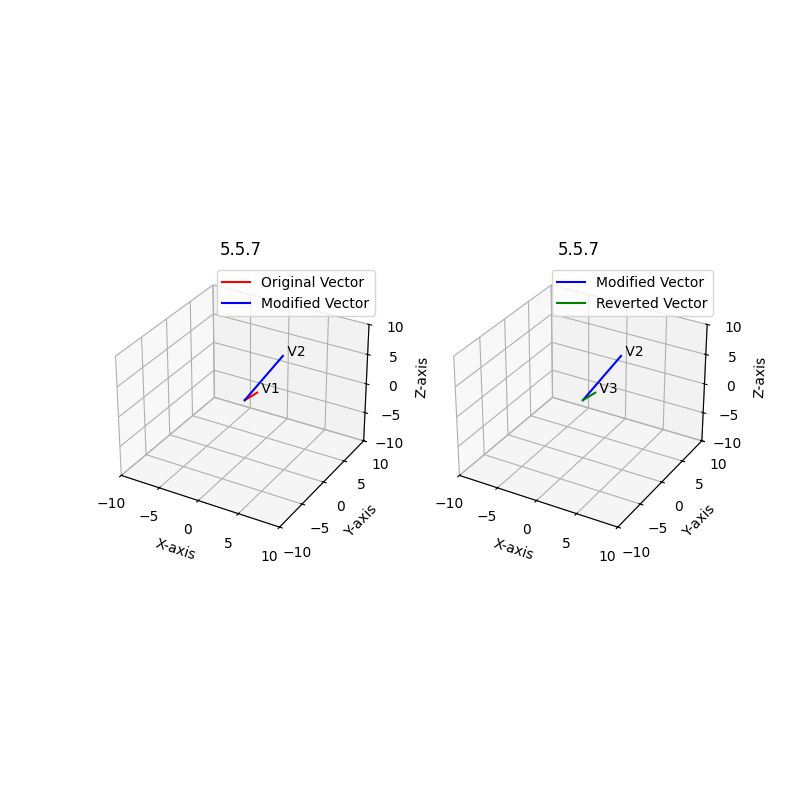
\includegraphics{figs/plot.png}
    \caption*{}
    \label{fig:plot}
\end{figure}
\end{document}
